\chapter{Manifolds and Coordinates}
  \begin{definition}[$C^k$ Functions]
    A function $f: \mathbb{R}^n\rightarrow \mathbb{R}^n$ is said to be in $C^k$ if all its partial derivatives up to and including order $k$ exist and are continuous.
  \end{definition}
  \begin{remark}
    When $k\rightarrow \infty$, the function $f: \mathbb{R}^n\rightarrow \mathbb{R}^n$ is said to be smooth, or in $C^{\infty}$.
  \end{remark}
  \section{Topological and Differentiable Manifolds}
    \begin{definition}[Topological Manifold\footnote{For a precise meaning
    of the terms "Hausdorff","Neighbourhood", "Homeomorphic", wait for
    chapter \ref{chapter:Basic Topology} to be done.}]
      A topological manifold is a Hausdorff space such that every point has a
      neighbourhood homeomorphic to $\mathbb{R}^n$.
    \end{definition}
    \begin{remark}
      A manifold that is locally homeomorphic to $\mathbb{R}^n$ is said to have dimension $n$.
    \end{remark}
    Since every point on the manifold has a neighbourhood homeomorphic to
    $\mathbb{R}^n$, locally the neighbourhood on the manifold "inherits"
    the metric topology of $\mathbb{R}^n$. I.e, the local homeomorphism to
    $\mathbb{R}^n$ implies the existence of open sets on the manifold, and
    because a homeomorphism is by definition bijective, there is a
    one-to-one correspondence between open sets in the neighbourhood and
    open sets in $\mathbb{R}^n$.

    In short, "locally" (in the neighbourhood of a point), the manifold has
    the same topology as $\mathbb{R}^n$.

    By the way, the manifold "inheriting" the metric topology of
    $\mathbb{R}^n$ locally is a very different concept from the idea of a
    metric tensor. So far, no metric has been defined on the manifold yet!

  \section{Charts}
    \begin{definition}[Chart]
      A chart $(U, \phi)$ of a manifold $\mathcal{M}$ is an open set U of $\mathcal{M}$, called the domain of the chart, together with a homeomorphism $\phi: U \rightarrow V$ of $U$ onto an open set $V$ in $\mathbb{R}^n$
    \end{definition}
    I.e, for an arbitrary $p\in U \subset \mathcal{M}$, we have $\phi(p) =
    \left(x^1(p), x^2(p),...,x^n(p)\right) \in \mathbb{R}^n$. We say that
    $p \in U$ has coordinates $\phi(p)$ in the chart $(U, \phi)$.

    In Physics terms, we would call $\left\{x^i(p)\right\}_{i = 1,...n}$
    the coordinate functions, and we would call the chart $(U, \phi)$ a
    local coordinate system.
  \section{Atlas}
    \begin{definition}[Atlas]
      \label{defn: Atlas definiton}
      An atlas of class $C^k$ on a manifold $\mathcal{M}$ is a set (i.e
      family) $\{(U_\alpha,\phi_\alpha)\}_{\alpha \in I}$\footnote{Note
      that $I\subset \mathbb{R}$} of charts of $\mathcal{M}$ such that the
      following holds:
      \begin{enumerate}
        \item{M is covered by the family in the sense that
          \begin{equation*}
            \mathcal{M} = \bigcup_{\alpha\in I} U_\alpha
          \end{equation*}}
        \item{\label{item:atlas defn}The maps $\phi_\beta \circ
        \phi_\alpha^{-1}: \phi_\alpha(U_\alpha \cap U_\beta) \rightarrow
        \phi_\beta(U_\alpha \cap U_\beta)$ are maps of open sets of
        $\mathbb{R}^n$ into $\mathbb{R}^n$ of class $C^k$.}
      \end{enumerate}
    \end{definition}
      Let's spend more time looking at property \ref{item:atlas defn} of
      defintion \ref{defn: Atlas definiton}.
      \begin{figure}[ht]
        \centering
        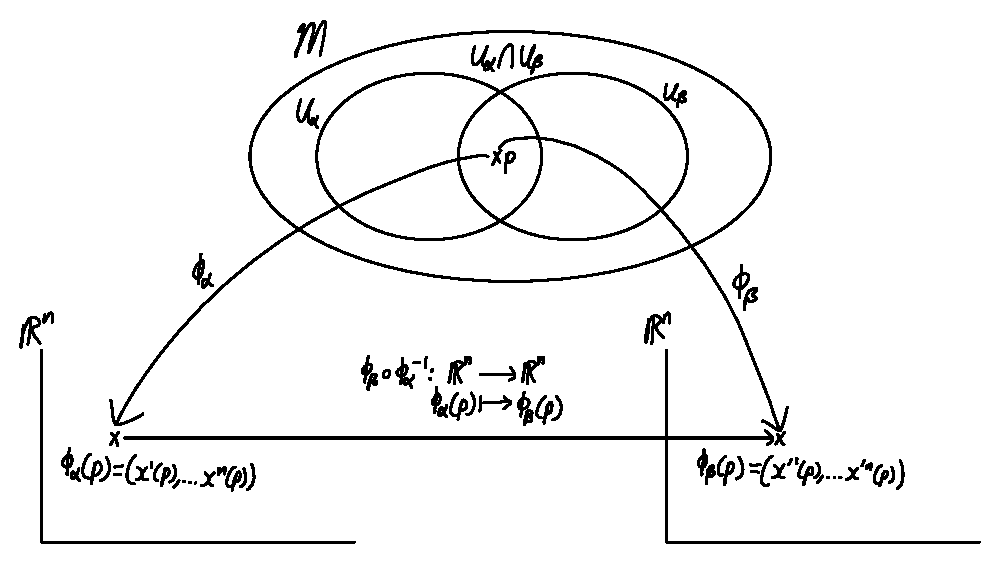
\includegraphics[width=0.7\textwidth, trim={0cm 0cm 0cm 0cm},clip]{Atlas defn}
        \caption[]{}
        \label{fig:atlas defn}
      \end{figure}
      With reference to Figure~\ref{fig:atlas defn}, consider a point $p
      \in U_\alpha \cap U_\beta$. $p$ has coordinates $\phi_\alpha(p)$ in
      the chart $(U_\alpha,\phi_\alpha)$, but has coordinates
      $\phi_\beta(p)$ in the chart $(U_\beta,\phi_\beta)$. These two charts
      induce a map\footnote{$\phi_\alpha^{-1}$ exists because $\phi_\alpha$ is a homeomorphism.} $\phi_\beta \circ \phi_\alpha^{-1}$ from
      $\phi_\alpha(U_\alpha \cap U_\beta) \subset \mathbb{R}^n$ to
      $\phi_\beta(U_\alpha \cap U_\beta) \subset \mathbb{R}^n$. Now, the
      map $\phi_\beta \circ \phi_\alpha^{-1}$ is actually $n$ coordinate
      transformation functions $\{x^{\prime i} = x^{\prime
      i}(x^1,...,x^n)\}_{i=1,...n}$. Thus, when we say that the map
      $\phi_\beta \circ \phi_\alpha^{-1}$ is of class $C^k$, we are saying
      that those $n$ coordinate transformation functions are also of class
      $C^k$.

      Two charts $(U_\alpha,\phi_\alpha)$, $(U_\beta,\phi_\beta)$ that satisfy the property are said to be $C^k$ compatible.

      \begin{definition}[Equivalent Atlases]
        Two $C^k$ atlases $\mathcal{F} = \{(U_\alpha,\phi_\alpha)\}_{\alpha
        \in I}$ and $\mathcal{G} =
        \{(U_{\alpha^\prime},\phi_{\alpha^\prime})\}_{\alpha^\prime \in I}$
        are equivalent\footnote{"Equivalent" here refers to equivalence relation, so we can form equivalence classes.} if every pair of charts $(U_\alpha,\phi_\alpha) \in
        \mathcal{F}$ and $(U_{\alpha^\prime},\phi_{\alpha^\prime}) \in
        \mathcal{G}$ are $C^k$ compatible.
      \end{definition}
      \begin{remark}
        An equivalent definiton (can be proved) is: Two $C^k$ atlases $\mathcal{F} = \{(U_\alpha,\phi_\alpha)\}_{\alpha
        \in I}$ and $\mathcal{G} =
        \{(U_{\alpha^\prime},\phi_{\alpha^\prime})\}_{\alpha^\prime \in I}$
        are equivalent if their union $\mathcal{F} \cup \mathcal{G}$ is a $C^k$ atlas.
      \end{remark}
  \section{Differentiable Manifold}
    \begin{definition}[Differentiable Manifold]
      A topological manifold $\mathcal{M}$ together with an equivalence
      class of $C^k$ atlases is a $C^k$ structure on $\mathcal{M}$; we say
      that $\mathcal{M}$ is a $C^k$ manifold or a differentiable manifold.
    \end{definition}
    \begin{remark}
      Very often, we want $k \rightarrow \infty$, so we can define tensor
      fields on $\mathcal{M}$. In this case, the manifold is called a smooth manifold.
    \end{remark}
  \section{Key Idea Behind Differential Geometry}
    In Physics, most of the time the variables that we are concerned with
    such as time, position, etc are all either elements of $\mathbb{R}$
    or $\mathbb{C}$, and our physical laws themselves are usually
    differential equations. Yet we know that the laws of Physics are
    independent of the choice of coordinates used. Thus, differential
    geometry is a natural language for expressing the laws of Physics.
    When we model our physical system with a differentiable manifolds, we
    can do calculus because locally the manifold looks like
    $\mathbb{R}^n$. But our results are also coordinate independent,
    because we can freely switch between coordinates due to the $C^k$
    structure; we just have to use the chain rule to do so.

    By the way, from here on, we deal strictly with differentiable or smooth manifolds.
  \section{Diffeomorphisms}
    \label{sec: Diffeomorphism}
    \begin{definition}[Differentiable Maps between Manifolds]
      \label{defn: differentiable map}
      Let $\mathcal{M}$, $\mathcal{N}$ be two $C^k$ differentiable
      manifolds of dimensions $m$ and $n$ respectively. Let $\mathcal{M}$
      have an atlas $\{(U_\alpha, \phi_\alpha)\}_{\alpha\in I}$\footnote{We
      will slowly drop the $"\alpha\in I"$ label for ease of notation...},
      and $\mathcal{N}$ have an atlas $\{(V_\beta, \psi_\beta)\}_{\beta\in
      I}$. Let $f$ be a map from $\mathcal{M}$ to $\mathcal{N}$.
      
      The map $f$ is said to be $C^r$ differentiable at $p\in\mathcal{M}$,
      $r\leq k$ if the $n$ coordinate transforms induced by $F \equiv \psi
      \circ f \circ \phi^{-1}$ are $C^r$ differentiable at $\phi(p)$, where
      $(U,\phi) \in \{(U_\alpha, \phi_\alpha)\}$ is a chart such that $p
      \in U$ and $(V,\psi) \in \{(V_\beta, \psi_\beta)\}$ is a chart such
      that $f(p) \in V$.
      
      If $f$ is differentiable $\forall p \in \mathcal{M}$, then $f$ is a
      differentiable map.
    \end{definition}
    \begin{remark}
      In definition~\ref{defn: differentiable map}, two particular charts
      $(U,\phi)$, $(V,\psi)$ are chosen. Yet it doesn't matter which charts
      we choose. Consider two other charts $(U^\prime,\phi^\prime)$ and
      $(V^\prime,\psi^\prime)$ such that $p \in U^\prime$, $f(p) \in
      V^\prime$. Consider $F^\prime = \psi^\prime \circ f \circ
      \phi^{\prime -1}$. Note that we can write\footnote{This trick of
      inserting an identity map $(\psi^{-1} \circ \psi)$ is a very useful
      trick, especially in proofs.} $F^\prime = \psi^\prime \circ
      (\psi^{-1} \circ \psi) \circ f \circ (\phi^{-1} \circ \phi) \circ
      \phi^{\prime -1} = (\psi^\prime \circ \psi^{-1}) \circ F \circ (\phi
      \circ \phi^{\prime -1})$, and because of the $C^k$ structure of the
      differentiable manifold, both $(\psi^\prime \circ \psi^{-1})$ and
      $(\phi \circ \phi^{\prime -1})$ are both $C^k$ functions. Thus, if
      $F$ is a $C^r$ function, then $F^\prime$ is also a $C^r$ function.
    \end{remark}
    \begin{figure}[h]
      \centering
      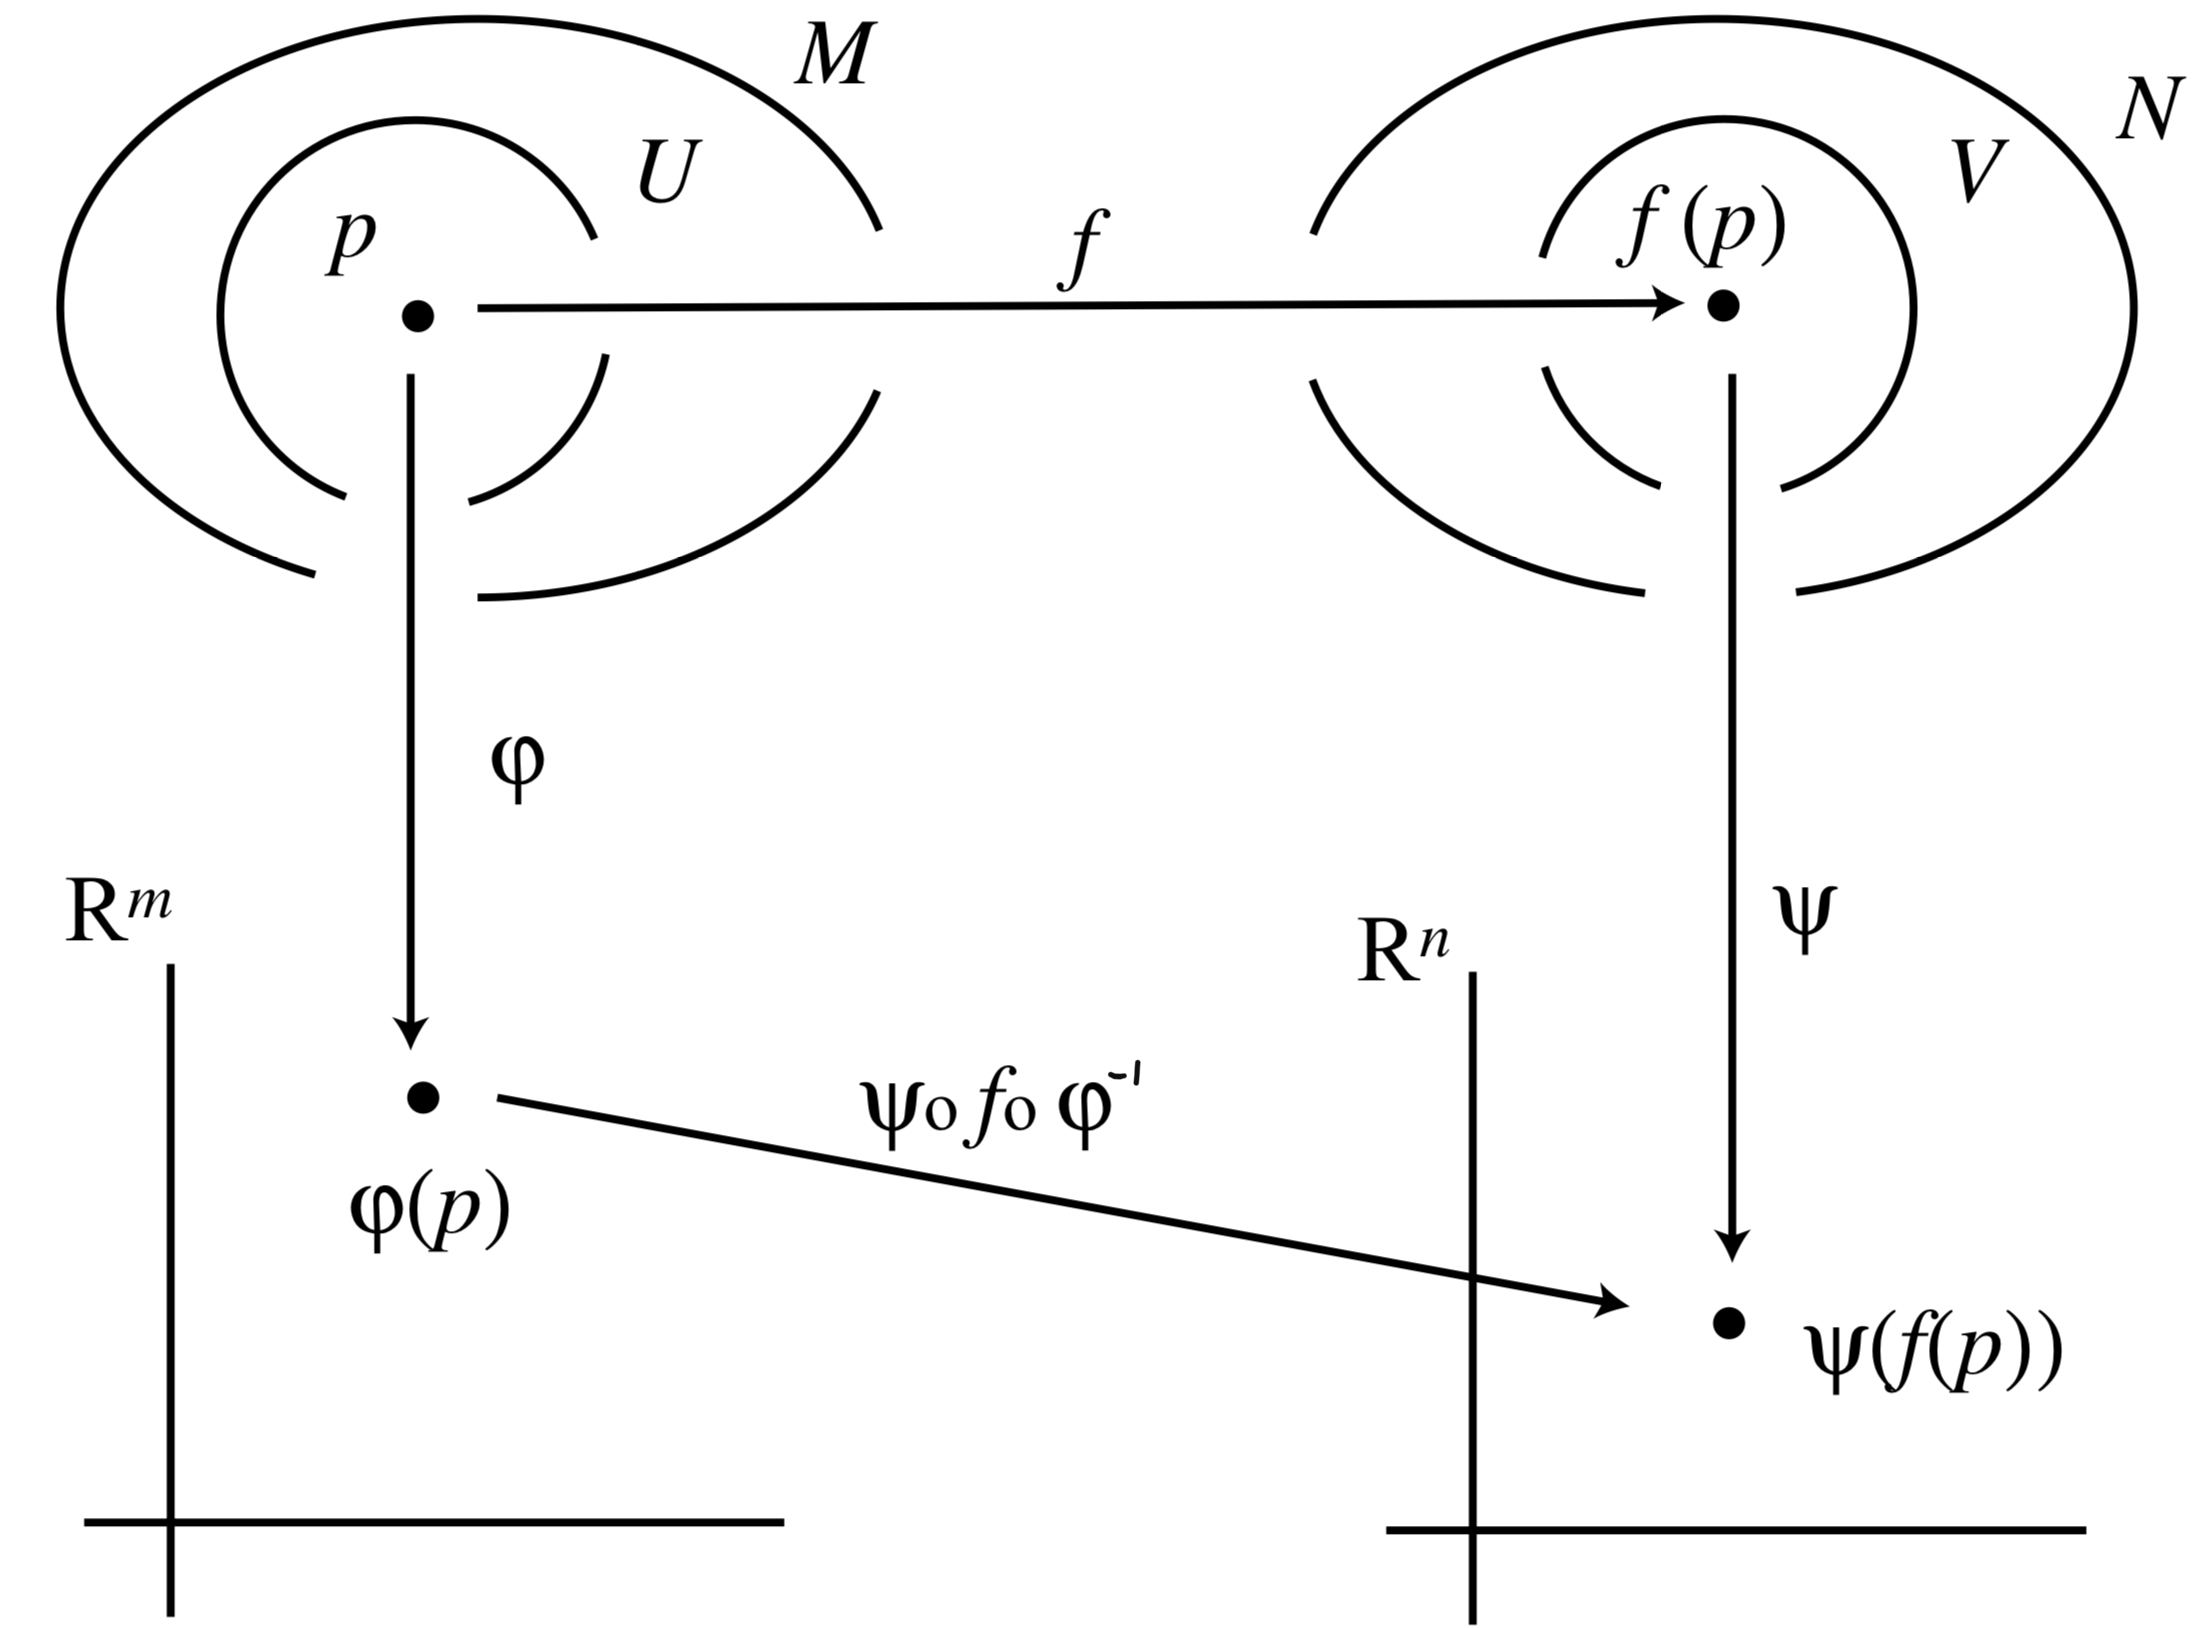
\includegraphics[width=0.6\textwidth, trim={0cm 0cm 0cm 0cm},clip]{Differentiable Map defn}
      \caption[]{Figure copied from Nakahara}
      \label{fig: differentiable map defn}
    \end{figure}
    Let's try to make sense of the above definition. With reference to
    Figure~\ref{fig: differentiable map defn}, consider a point $p\in
    \mathcal{M}$ and its image under $f$, i.e $f(p) \in \mathcal{N}$.
    Consider two charts, $(U,\phi) \in \{(U_\alpha, \phi_\alpha)\}$ and
    $(V,\psi) \in \{(V_\beta, \psi_\beta)\}$ such that $p \in U$ and $f(p)
    \in V$. Then, $F = \psi \circ f \circ \phi^{-1}$ is a map from $\phi(U)
    \subset \mathbb{R}^n$ to $\psi(V)\subset \mathbb{R}^m$. In fact, we see
    that $F$ induces $n$ coordinate transformation functions; if we let
    $\phi(p) = \left(x^1,...,x^m\right)$, then $\psi(f(p)) =
    \left(x^{\prime 1},...x^{\prime n}\right) = \left(x^{\prime
    1}(x^1,...,x^m),...x^{\prime n}(x^1,...,x^m)\right)$. Then, for $f$ to be a differentiable map, these $n$ coordinate functions have to be $C^r$.
    \begin{definition}[Diffeomorphism]
      A map $f:\mathcal{M} \rightarrow \mathcal{N}$, where $\mathcal{M}$ and
      $\mathcal{N}$ are $C^k$-differentiable manifolds of dimensions $m$ and
      $n$ respectively, is said to be a diffeomorphism if:
      \begin{enumerate}
        \item{$f$ is bijective $(\implies m = n)$.}
        \item{$f$ and $f^{-1}$ are both $C^r$ functions.}
      \end{enumerate}
    \end{definition}